% !TEX encoding = UTF-8 Unicode
\documentclass[fontsize=11pt,paper=a4,titlepage,twoside,DIV=calc,draft=false]{scrbook}
% 11pt: Normale Textkörpergröße
% a4paper: Größe des Druckmediums
% titlepage: Titel auf einer separaten Seite ohne Seitenzahl
% twoside: Zweiseitiges Layout
% openright: Kapitel beginnen immer auf der rechten Seite
% headsepline: Trennt Textkörper von Headings durch Strich (entspr.: /footsepline)
% headinclude,footinclude: Kopf- und Fußzeile zählen zum Textkörper
% DIV=calc: Für die gewählten Optionen wird ein optimales Seitenverhältnis errechnet
% draft=true: Für Bilder wird die Box freigehalten, erheblicher Geschwindigkeitsvorteil.
% abstract: Setzt den Titel 'Zusammenfassung' vor den abstract

\usepackage{blindtext} 
\usepackage{upgreek}
%\usepackage{subfigure}

%  %  %  %  Bindungskorrektour  %  %  %  %
\KOMAoptions{BCOR=10mm}  


%  %  %  %  Abkürzungen  %  %  %  %
% Das Einführen dieser Befehler verhindert Umbrüche bei mehrgliedrigen Abkürzungen
\usepackage{xspace}
\newcommand{\zB}{\mbox{z.\,B.}\xspace}
% Abkürzung für zum Beispiel


%  %  %  %  Einheiten  %  %  %  %
\usepackage[thinspace,thinqspace,squaren,textstyle]{SIunits}
% Komfoatables Paket zum Einbinden von Einheiten


%  %  %  %  Kodierung, Schrift und Sprache  %  %  %  % 
\usepackage[utf8]{inputenc}
\usepackage{palatino}
\usepackage[ngerman]{babel}
% damit man Text aus dem PDF korrekt rauskopieren kann


%  %  %  %  Grafiken, Tabellen, Mathematikumgebungen  %  %  %  %
\usepackage{graphicx}
\usepackage{tabularx}
\usepackage{xcolor}
\definecolor{halfgray}{gray}{0.55} 
\usepackage{amsmath,amsfonts,amssymb}
\usepackage{flafter,afterpage}
\usepackage[section]{placeins}
\usepackage{setspace} \onehalfspacing
\usepackage[margin=8mm,font=small,labelfont=bf,format=plain]{caption}
\usepackage[margin=8mm,font=small,labelfont=bf,format=plain]{subcaption}

\numberwithin{equation}{chapter}
\numberwithin{figure}{chapter}
\numberwithin{table}{chapter}


%  %  %  %  Kopf- und Fußzeilen  %  %  %  %

\renewcommand\frontmatter{\pagenumbering{Roman}}
\usepackage{chngcntr} 
\counterwithout{footnote}{chapter}
  
  
% Zeilenabstand zwischen zwei Fußnoten:
\footnotesep9pt
% Einrücken der Fußnoten:
\deffootnote[1.5em]{1em}{1.5em}{\thefootnotemark\ \ }

\usepackage{fancyhdr}				% Paket für leicht konfigurierbare Kopf- und Fußzeilen
\fancypagestyle{plain}{				% Neue Gestaltung der Chapter- Page
\fancyhf{} 							% Clear all header and footer fields
\renewcommand{\headrulewidth}{0pt}	% Keine Trennlinie zwischen Kopf- / Fußzeile und Textkörper
\renewcommand{\footrulewidth}{0pt}}

\fancypagestyle{myfoot}{			% Neue Gestaltung der frontmatter pages
\fancyhf{}							% Clear all header and footer fields
\fancyhead[RO]{\thepage}			% Seitenzahl außen auf ungeraden Seiten
\fancyhead[LE]{\thepage}			% Seitenzahl außen auf geraden Seiten
\renewcommand{\headrulerwidth}{0pt}	% Keine Trennlinie zwischen Kopf- / Fußzeile und Textkörper
\renewcommand{\footrulerwidth}{0pt}}

\pagestyle{fancy}					% Pagestyle fancy aktiviert selbstkonfigurierten Style
\fancyhf{} 							% Alle Kopf- und Fußzeilenfelder werden zunächst bereinig
\renewcommand{\headrulewidth}{0pt}	% Keine Trennlienie zwischen Kopfzeile und Textkörper

\renewcommand{\chaptermark}[1]{\markboth{#1}{}}
%\renewcommand{\sectionmark}[1]{\markright{#1}{}}

\fancyhead[RO]{\leftmark ~~~~ \thepage}
\fancyhead[LE]{\thepage ~~~~ \nouppercase \rightmark}


%  %  %  %  Überschriften  %  %  %  %


%  %  %  %  Verzeichnisse  %  %  %  %

% % % Literaturverzeichnis % % %
%\usepackage{natbib}	

% % % Inhaltsverzeichnis % % %
% Die Chaptereinträge:
\usepackage{titletoc}

\titlecontents{chapter}
				[0pc]
				{\addvspace{0.5pc}%			
				%\filouter}
				}
				{\sffamily\LARGE\thecontentslabel\quad\sffamily\LARGE}{}
				{\titlerule*[0.75pc]{}\enskip\rmfamily\LARGE}%\contentspage}  % Wäre mit Seitenzahl 																					rechtsbündig
				[\addvspace{.5pc}]

% Die Sectioneinträge:
\titlecontents{section}
[3.78em]
{}
{\rmfamily\contentslabel{2.3em}\rmfamily}
{\hspace*{-2.3em}}
{\titlerule*[0.75pc]{.}\enskip\contentspage}
[\addvspace{.1em}]

% Die Subsectioneinträge:
\titlecontents{subsection}
[6.2em]
{}
{\rmfamily\contentslabel{2.3em}\rmfamily}
{\hspace*{-2.3em}}
{\titlerule*[0.75pc]{.}\enskip\contentspage}
[\addvspace{.1em}]

%\titlecontents{subsection}
%[6.8em]
%{}
%{\rmfamily\normalsize\contentslabel{3em}\rmfamily\large}
%{\hspace*{-2.3em}}
%{\titlerule*[0.75pc]{.}\enskip\contentspage}
\begin{document}

%  %  %  %  Titelseite  %  %  %  %
\begin{titlepage}
	\begin{tabularx}{\linewidth}{X}		
 		
		\\ \\ \hline	
 		 			
		\vspace{2em}
		
  		\begin{singlespace}
  			\begin{center}    \Large	\bfseries 
  				Software Engineering 
  			\end{center}
  		\end{singlespace}
  		
  		\vspace{2em}
  		
  		\begin{singlespace}
  			\begin{center}	\bfseries 
   				Anforderungsanalyse zur Entwicklung 
				eines SW-Systems zur Unterstützung 
				der Einführung von Gleitarbeitszeit
  			\end{center}
  		\end{singlespace} 
		
		\vspace{18em}
		
  		\begin{center}
  			vorgelegt von \\ 
			\vspace{2em}
 			Tom Graupner \\
			Markus Klemm \\
			Leonard Hecker 
  		\end{center}
		
		\vspace{2em}
		
		\\ \\ \hline
		
	\end{tabularx}
\end{titlepage}

%  %  %  %  Inhaltsverzeichnis  %  %  %  %

\tableofcontents

%  %  %  %  Hauptteil  %  %  %  %
\mainmatter

\chapter{Einführung}
Das Unternehmen \textsc{EKS}\footnote{Abkürzung für \textsc{Entwicklung von kundenspezifischer Software}} evaluiert aktuell die Umstellung ihres Arbeitszeitmodells zur Gleitzeit. Die Erfassung und Auswertung der Arbeitszeit soll dabei durch ein Software-System unterstützt werden. Die vorliegende Anforderungsanalyse beschäftigt sich zunächst mit den Rahmenbedingung und den Funktionen, die vom System übernommen werden sollen. Neben der Zusammenfassung aller funktionalen Anforderungen und der Struktur der Eigangs- und Ausgangsdaten, enthält diese Analyse verschiedene Anwendungsfalldiagramme\footnote{Als Abk\"urzung wird im folgenden \textsc{AWD} verwendet. Daran angelehnt ist die Abk\"urzung \textsc{AWF} f\"ur einen Anwendungsfall}, sowie ein Entity Relationship Model, welches die Speicherung der Daten veranschaulicht.

\chapter{Dokumentation der Anforderungen}
Anforderungen an ein Software-Produkt werden im Allgemeinen zunächst in funktionale und nicht-funktionale Anforderungen unterteilt. Erstere decken dabei die Fähigkeiten und die Beschaffenheiten ab, die der Benutzer der Software zur Problemlösung oder zur Erreichung seines Zieles benötigt. Nicht-funktionale Anforderungen unterteilen sich weiterhin in Rahmenbedingungen und Qualitätsanforderungen.

\section{Funktionale Anforderungen}
Die folgende Auflistung enth\"alt die groben Funktionen, die vom Software-System erf\"ullt werden sollen. Bei einigen handelt es sich dabei um \textit{abstrakte Funktionen}, welche sich im weiteren Verlauf der Analyse feiner aufgliedern werden.

\begin{itemize}
	\item \textbf{Anwesenheit erfassen} \textit{\guillemotleft \ abstrakt \ \guillemotright}
	\item \textbf{Urlaub planen - Mitarbeiter} \textit{\guillemotleft \ abstrakt \ \guillemotright}
	\item \textbf{Urlaub verwalten - Abteilungsleiter} \textit{\guillemotleft \ abstrakt \ \guillemotright}
	\item \textbf{Krankheitsdaten erfassen}
	\item \textbf{Anwesenheit auswerten}
	\item \textbf{Zeitauswertung f\"ur Abteilungsleiter} \textit{\guillemotleft \ abstrakt \ \guillemotright}
\end{itemize} 

\subsection{Tabellarischer \"Uberblick}
Die folgenden Tabellen fassen nun alle voneinander unabh\"angigen funktionalen Anforderungen an das Software-System zusammen.  Im Rahmen der Anforderungsanalyse verwendet man f\"ur unabh\"angige funktionale Anforderungen ebenfalls den Begriff  \textit{essentielle Funktionen}.

{
\vspace{1cm}
\hspace{-3,5cm}
\footnotesize
\begin{tabular}{|p{3cm}|p{4cm}|p{4cm}|p{4cm}|p{2cm}|}
	\hline
		\textbf{Funktion	} &	
		\textbf{Eingangsdaten} &
		\textbf{Ausgangsdaten}& 
		\textbf{Bemerkungen}	&
		\textbf{abstrakter AWD} \\
	\hline \hline 
		\textit{Betreten} &
		MA-ID und Uhrzeit &
		Zutritt und Speicherung der Zeit, alternativ Zutrittsverweigerung & 
		Bei einer ung\"ultigen MA-ID kann der Zutritt verweigert werden &  
		\textbf{Anwesenheit erfassen} \\
	\cline{1-4}
		\textit{Verlassen} & 
		MA-ID und Uhrzeit & 
		Verlassen und Speicherung der Zeit, alternative Fehlermeldung &
		& 
		\\
	\cline{1-4}
		\textit{Wachdienst \mbox{informieren}} &
		Mitarbeiterliste &
		Detaillierte Information an den Wachdienst &
		Der Wachdienst wird st\"undlich dar\"uber informiert, welche Mitarbeiter sich im Geb\"aude befinden &
		\\
	\hline
\end{tabular}
}

{
\vspace{0,5cm}
\hspace{-3,5cm}
\footnotesize
\begin{tabular}{|p{3cm}|p{4cm}|p{4cm}|p{4cm}|p{2cm}|}
	\hline
		\textit{Urlaub beantragen} & 
		Urlaubswunsch & 
		Urlaubsantrag & 
		Urlaub wird unter Verwendung der eigenen MA-ID beim jeweiligen Abteilungsleiter beantragt & 
		\textbf{Urlaub \newline planen, \newline  Mitarbeiter } \\
	\cline{1-4}
		\textit{Urlaubsinformationen anzeigen} & 
		Wunsch nach Urlaubsinformationen & 
		Informationen zu Urlaubsterminen, Beantragungs\-status, verbrauchten und verbleibenden Urlaubstagen &  
		&  
		\\
	\cline{1-4}
		\textit{Urlaubsantrag \newline stornieren} &
		Storno-Wunsche &
		Storno-Best\"atigung mit Aktualisierung der Urlaubsdaten &
		Mitarbeiter kann offene, abgelehnte und genehmigte (noch nicht angetretene) Urlaubsantr\"age stornieren &
		\\
	\cline{1-4}
		\textit{Urlaubsvorschlag annehmen} &
		Urlaubsvorschlag des Abteilungsleiter &
		 Aktualisierung der Urlaubsinformationen &
		Abteilungsleiter k\"onnen Mitarbeiter ihrer Abt. Vorschl\"age unterbreiten &
		\\
	\cline{1-4}
		\textit{Urlaubsvorschlag \newline stornieren} &
		Urlaubsvorschlag des Abteilungsleiter und Storno-Wunsch &
		Stornierungsmitteilung und Aktualisierung der Urlaubsinformationen &
		Abteilungsleiter k\"onnen Mitarbeitern ihrer Abt. Vorschl\"age unterbreiten &
		\\
	\hline
\end{tabular}
}

{
\hspace{-3,5cm}
\footnotesize
\begin{tabular}{|p{3cm}|p{4cm}|p{4cm}|p{4cm}|p{2cm}|}
	\hline 
		\textbf{Funktion	} &	
		\textbf{Eingangsdaten} &
		\textbf{Ausgangsdaten}& 
		\textbf{Bemerkungen}	&
		\textbf{abstrakter AWD} \\
	\hline \hline 
		\textit{Urlaubsantrag \newline genehmigen} &
		Urlaubsantrag eines MA &
		Aktualisierung der Urlaubsdaten und Best\"atigung &
		Abteilungsleiter m\"ussen Antr\"age ihrer Mitarbeiter genehmigen &
		\textbf{Urlaub \newline verwalten, \newline  Abt.-Leiter } \\
	\cline{1-4}
		\textit{Urlaubsantrag \newline ablehnen} &
		Urlaubsantrag eines MA &
		Aktualisierung der Urlaubsdaten und Absage&
		Abteilungsleiter k\"onnen Antr\"age ihrer Mitarbeiter ablehnen &
		\\
	\cline{1-4}
		\textit{Vorschlag \newline unterbreiten} &
		Urlaubsvorschlag des Abteilungsleiters &
		Urlaubsvorschlag an Mitarbeiter und Aktualisierung der Urlaubsinformationen &
		Abteilungsleiter k\"onnen Mitarbeitern Urlaubsvorschl\"age unterbreiten &
		\\
	\cline{1-4}
		\textit{Urlaubsinformationen eines Mitarbeiters an\-zeigen} &
		Wunsch des Abteilungsleiters nach Urlaubsinformationen eines Mitarbeiters &
		Detaillierte Informationen zur Abteilung &
		Abteilungsleiter k\"onnen sich zur Entscheidungs\-unterst\"utzung die Urlaubs\-informationen eines Mitarbeiters anzeigen lassen &
		\\
	\hline
\end{tabular}
}

{
\vspace{0,5cm}
\hspace{-3,5cm}
\footnotesize
\begin{tabular}{|p{3cm}|p{4cm}|p{4cm}|p{4cm}|p{2cm}|}
	\hline 
		\textit{Krankmeldung \newline erfassen} &
		Krankenschein eines Mitarbeiters &
		Aktualisierung der Urlaubsinformationen &
		Sachbearbeiter (HR) erfasst Krankmeldungen von Mitarbeitern und betroffene Urlaubsinformationen werden sofort aktualisiert &
		 \\
	\hline	
\end{tabular}
}

{
\vspace{0,5cm}
\hspace{-3,5cm}
\footnotesize
\begin{tabular}{|p{3cm}|p{4cm}|p{4cm}|p{4cm}|p{2cm}|}
	\hline 
		\textit{Anwesenheit \newline auswerten} &
		Anwesenheitsinformationen eines Mitarbeiters &
		Detaillierte Arbeitszeit\-aus\-wertung  des Mitarbeiters &
		Die Auswertung wird w\"ochentlich automatisch erstellt und dem Mitarbeiter per Email zugesandt &
		 \\
	\hline	
\end{tabular}
}

{
\hspace{-3,5cm}
\footnotesize
\begin{tabular}{|p{3cm}|p{4cm}|p{4cm}|p{4cm}|p{2cm}|}
	\hline
		\textbf{Funktion	} &	
		\textbf{Eingangsdaten} &
		\textbf{Ausgangsdaten}& 
		\textbf{Bemerkungen}	&
		\textbf{abstrakter AWD} \\
	\hline \hline 
		\textit{Gesamtbilanz \newline anfordern} &
		Wunsch nach Gesamtbilanz &
		Gesamtbilanz enth\"alt detaillierte Informationen zur Arbeits\-zeit\-auswertung der Abteilung &
		Die Kennzahlen sind absolut und prozentual angegeben und betreffen einen beliebigen, abgelaufenen Zeitraum &
		\textbf{Zeitaus\-wertung f\"ur Abt.-Leiter}\\
	\cline{1-4}
		\textit{Urlaubszeitbilanz \newline anfordern} &
		Wunsch nach Urlaubsbilanz &
		Urlaubszeitbilanz ente\"alt beantragte Urlaubstage der Abteilung in einem vorausschauenden Zeitraum &
		Antr\"age werden absolut und prozentual bezogen auf die Gesamtarbeitszeit dargestellt &
		\\ 
	\cline{1-4}
		\textit{Anwesenheitsliste \newline anfordern}&
		Wunsch nach Anwesenheitsliste &
		Liste enth\"alt alle momentan anwesenden Mitarbeiter der eigenen Abteilung &
		&
		\\
	\hline
\end{tabular}
}

\vspace{1cm}

\subsection{Struktur der Eingangs- und Ausgangedaten}
Jede essentielle Funktion besitzt definierte Eingangs- und Ausgangsdaten. Die folgende Auflistung stellt die Struktur der entsprechenden Daten aller zuvor genannten essentiellen Funktionen dar.

{
\vspace{1cm}
\hspace{-2cm}
\footnotesize
\begin{tabular}{|p{3cm}|p{6cm}|p{6cm}|}
	\hline
		\textbf{Funktion	} &	
		\textbf{Struktur der Eingangsdaten} &
		\textbf{Struktur der Ausgangsdaten} \\
	\hline \hline
		\textit{Betreten} &
		+ MA-ID \newline + Uhrzeit &
		Best\"atigung des Zutritts und \newline Datensatz :=\{MA-ID, Uhrzeit\}, \newline alternativ Fehlermeldung \\
	\hline
		\textit{Verlassen} &
		+ MA-ID \newline + Uhrzeit &
		Best\"atigung des Verlassen und \newline Datensatz :=\{MA-ID, Uhrzeit\}, \newline alternativ Fehlermeldung \\
	\hline
		\textit{Wachdienst \newline informieren} &
		St\"undlicher Trigger zum Ausl\"osen der Benachrichtigung&
		Detaillierte Mitarbeiterliste mit den Spalten \{MA-ID, Nachname, Vorname, B\"uro\} \\
	\hline 
\end{tabular}
}

\newpage
% \thispagestyle{empty}
{
\hspace{-2cm}
\footnotesize
\begin{tabular}{|p{3cm}|p{6cm}|p{6cm}|}
	\hline
		\textbf{Funktion	} &	
		\textbf{Struktur der Eingangsdaten} &
		\textbf{Struktur der Ausgangsdaten} \\
	\hline \hline		
	\textit{Urlaub beantragen} &
		Urlaubswunsch := \{MA-ID, Liste: zu beantragende Urlaubstage\}&
		Urlaubsantrag := \{MA-ID, Nachname, Vorname, Liste: zu beantragende Urlaubstage\}\\
	\hline
		\textit{Urlaubsinformationen anzeigen} &
		Wunsch nach Urlaubsinformationen &
		Urlaubsinformationen := \{verbrauchte Urlaubstage, verbleibende Urlaubstage, Liste: Urlaubstermine inkl. Status (offen, genehmigt, abgelehnt\}\\
	\hline		
		\textit{Urlaubsantrag \newline stornieren} &
		Urlaubsantrag s.o. (Status: offen / genehmigt und noch nicht angetreten).&
		Best\"atigung der Stornierung und aktualisierte Urlaubsinformationen := \{verbrauchte Urlaubstage, verbleibende Urlaubstage, Liste: Urlaubstermine inkl. Status (offen, genehmigt, abgelehnt\}\\
	\hline
		\textit{Urlaubsvorschlag \newline annehmen} &
		Urlaubsvorschlag := \{MA-ID, Liste: vorgeschlagener Urlaubstage \}&
		Best\"atigung des Urlaubsvorschlages und aktualisierte Urlaubsinformationen := \{verbrauchte Urlaubstage, verbleibende Urlaubstage, Liste: Urlaubstermine inkl. Status (offen, genehmigt, abgelehnt\}\\
	\hline
		\textit{Urlaubsvorschlag \newline stornieren} &
		Urlaubsvorschlag s.o.&
		Best\"atigung des Urlaubsvorschlages und aktualisierte Urlaubsinformationen := \{verbrauchte Urlaubstage, verbleibende Urlaubstage, Liste: Urlaubstermine inkl. Status (offen, genehmigt, abgelehnt\}\\
	\hline 
	\hline
		\textit{Urlaubsantrag \newline genehmigen} &
		Urlaubsantrag s.o. &
		Best\"atigung der Genehmigung und aktualisierte Urlaubsinformationen := \{verbrauchte Urlaubstage, verbleibende Urlaubstage, Liste: Urlaubstermine inkl. Status (offen, genehmigt, abgelehnt\}\\
	\hline
		\textit{Urlaubsantrag \newline ablehnen} &
		Urlaubsantrag s.o. &
		Best\"atigung der Ablehnung und aktualisierte Urlaubsinformationen := \{verbrauchte Urlaubstage, verbleibende Urlaubstage, Liste: Urlaubstermine inkl. Status (offen, genehmigt, abgelehnt\}\\
	\hline
		\textit{Urlaubsvorschlag \newline unterbreiten} &
		Wunsch einen Vorschlag zu unterbreiten oder konkreter Urlaubsantrag s.o.&
		Urlaubsvorschlag := \{MA-ID, Nachname, Vorname, Liste: vorgeschlagener Urlaubstage\} und aktualisierte Urlaubsinformationen := \{verbrauchte Urlaubstage, verbleibende Urlaubstage, Liste: Urlaubstermine inkl. Status (offen, genehmigt, abgelehnt\}\\
	\hline
		\textit{Urlaubsinformationen eines Mitarbeiters an\-zeigen} &
		Wunsch nach Urlaubsinformationen &
		Urlaubsinformationen := \{verbrauchte Urlaubstage, verbleibende Urlaubstage, Liste: Urlaubstermine inkl. Status (offen, genehmigt, abgelehnt\}\\
	\hline 
\end{tabular}
}

{
\hspace{-2cm}
\footnotesize
\begin{tabular}{|p{3cm}|p{6cm}|p{6cm}|}
	\hline
		\textbf{Funktion	} &	
		\textbf{Struktur der Eingangsdaten} &
		\textbf{Struktur der Ausgangsdaten} \\
	\hline \hline	
		\textit{Krankmeldung erfassen} &
		Krankenschein eines \newline Mitarbeiters := \{Nachname, Vorname, Geburtsdatum, Zeitraum der Bescheinigung\} &
		Entsprechende Aktualisierung der Mitarbeiterdatens\"atze f\"ur Urlaubstage, Soll- und Ist-Arbeitszeit \\
	\hline \hline
		\textit{Anwesenheit \newline auswerten} &
		Arbeitsstunden, Urlaubstage und Krankmeldungen des Mitarbeiters&
		Detaillierte Arbeitszeitauswertung :=\{Soll-Arbeitszeit, Ist-Arbeitszeit, Stand des Arbeitszeitkontos \} \\
	\hline \hline
		\textit{Gesamtbilanz \newline anfordern} &
		Wunsch nach Gesamtbilanz &
		Gesamtbilanz zu Abteilung :=\{Sollarbeitszeit, tats\"achliche Arbeitsstunden, Urlaubstage, Krankheitstage, \"Uberstunden\}\\
	\hline
		\textit{Urlaubsbilanz \newline anfordern} &
		Wunsch nach Urlaubsbilanz&
		Urlaubsbilanz der Abteilung :=\{beantragte Urlaubstage (absolut und prozentual bezogen auf Gesamtarbeitszeit)\}\\
	\hline
		\textit{Anwesenheitsliste \newline anfordern} &
		Wunsch nach Anwesenheitsliste &
		Anwesenheitsliste der Abteilung :=\{MA-ID, Nachname, Vorname, Arbeitsplatz\} \\
	\hline
\end{tabular}
}


\newpage
\section{Qualit\"atsanforderungen}
Nachdem weder interne, noch externe Qualit\"atsanforderungen explizit in den vorliegenden Rahmenbedingungen genannt sind, lautet die Aufgabe hier globale Anforderungen zu formulieren und eigene Gedanken zu entwickeln. \newline

Ein allgemeiner Punkt herausragender Bedeutung ist beispielsweise \newline \mbox{\textit{Datensicherheit und Integrit\"at}}. Aufgrund der Sensibilit\"at der zu verarbeitenden Daten und der mit ihnen verbundenen Business-Prozesse (e.g. Buchhaltung) ist unbedingt daf\"ur zu sorgen, dass jegliche Daten \textit{zugriffssicher,} \textit{redundant} und unter \textit{definierten Integrit\"atsbestimmungen} gespeichert und verarbeitet werden. \newline

F\"ur die sp\"atere Erweiterung oder Wartung der Software ist es au{\ss}erdem von gro{\ss}er Bedeutung, alle Funktionen und Komponenten des Systems l\"uckenlos zu dokumentieren. \newline
 
Geht man etwas ins Detail und betrachtet die essentiellen Funktionen, so gibt es Punkte an denen die Benutzerfreundlichkeit deutlich verbessert werden kann. Empfohlen w\"aren unter anderem \textit{Interaktionen mit der Software zu best\"atigen}. Gemeint ist damit, dem Benutzer R\"uckmeldung zu erfolgreich oder nicht erfolgreich abgeschlossenen Interaktionen zu geben. \newline

Weitere vorstellbare Qualit\"atsanforderungen werden nach Bedarf mit dem Auftraggeber abgesprochen.

\newpage
\section{Rahmenbedingungen}
Als abschlie{\ss}ender Punkt der schriftlichen Formulierung der Anforderungen werden die Rahmenbedingungen festgehalten. Hierbei unterscheidet man zwischen \textit{technologischen}, \textit{rechtlichen} und \textit{organisatorischen Rahmenbedingungen}. \newline

Zu den \textit{technischen Rahmenbedingungen} geh\"ort dabei, dass das System Zugriff auf den betriebsinternen Jahreskalender ben\"otigt. Dies ist notwendig, um Feiertage und Betriebsruhetage automatisch in die Bilanz der Arbeitszeit\-konten einbeziehen zu k\"onnen. Weiterhin sollen Urlaubstage und Krankmeldungen unmittelbar in die Bilanz einflie{\ss}en.  \newline

Wichtigster Teil der \textit{rechtlichen Rahmenbedingungen} ist zweifelsohne das Thema Datensicherheit. Die Vollst\"andigkeit und Integrit\"at der personenbezogenen Daten muss zu jedem Zeitpunkt gew\"ahrleistet sein. Dies ist notwendig um Rechtssicherheit zu schaffen, f\"ur den Arbeitgeber und den Arbeitnehmer.  \newline

Die \textit{organisatorischen Rahmenbedingungen} beinhalten vor allem Details zu den Arbeitszeitmodellen im Unternehmen. So besitzt ein Standard-Arbeitstag 8 Stunden und eine Arbeitswoche dementsprechenden 40 Stunden. Das Arbeitszeitkonto eines jeden Mitarbeiters wird dabei vom Beginn des Arbeitsverh\"altnisses an kumulativ gef\"uhrt.  

\newpage

\chapter{Kontextdiagramm}
Nach der ausf\"uhrlichen Formulierung der Anforderungen folgt nun die Modellierung des SW-Systems. In einer ersten Abstraktion zeigt Abbildung \ref{Kontext} das entsprechenden \textit{Kontextdiagramm}.  Es zeigt des System und dessen Schnittstellen zur Umwelt, sowie die Beziehungen zwischen den Benutzern.

\begin{figure}[hbp]
	\centering
	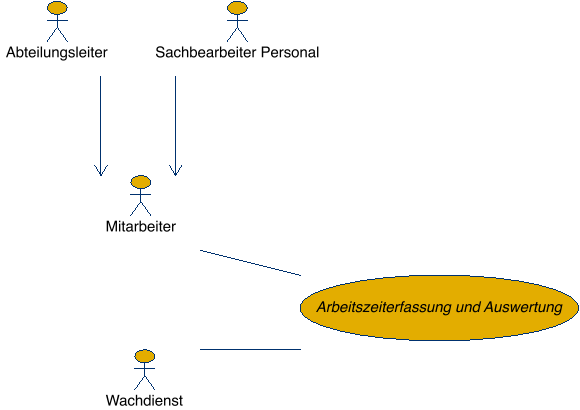
\includegraphics[width=0.9\linewidth]{UML/Export/Kontext.png}
	\caption{Kontextdiagramm zum SW-System \textit{Arbeitszeiterfassung und Auswertung}. Der Akteur Mitarbeiter generalisiert die Akteure Abteilungsleiter und Sachbearbeiter Personal}
	\label{Kontext}
\end{figure}

\chapter{Anwendungsfalldiagramme}
In einer weiteren Abstraktion werden die einzelnen Funktionen und ihre Kommunikationsbeziehungen zu den verschiedenen Akteuren dargestellt. 

\section{AWD der groben Funktionalität}
Abbildung \ref{AWD} zeigt die oberste Abstraktionsebene der Anwendungsfalldiagramme. Die enthaltenen \textit{abstrakten Funktionen} Kapseln dabei mehrere verwandte Anwendungsf\"alle.

\vspace{1cm}
\begin{figure}[hbp]
	\centering
	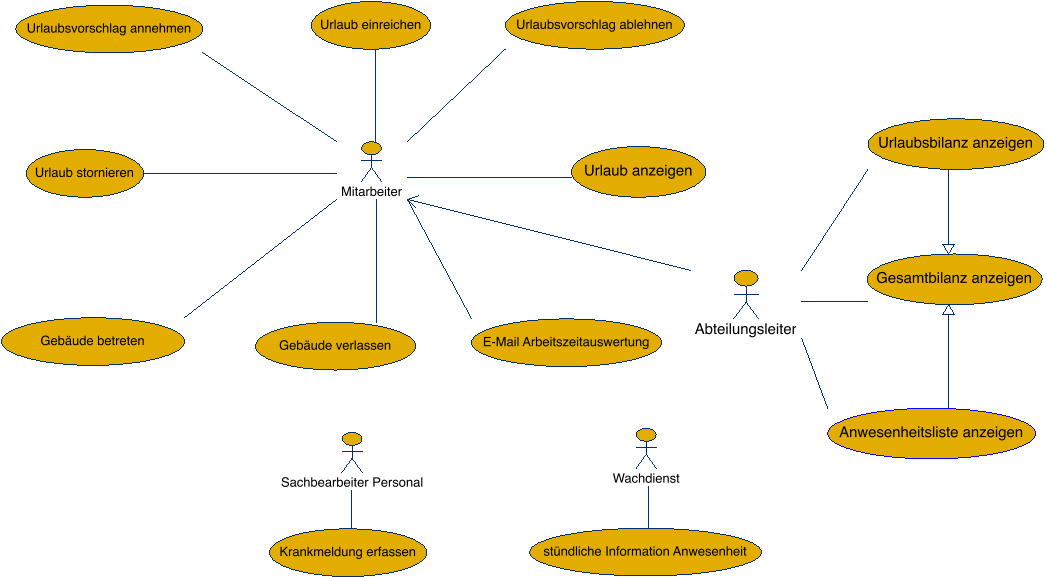
\includegraphics[width=\linewidth]{UML/Export/Grob.png}
	\caption{Anwendungsfalldiagramm zur groben \"Ubersicht.}
	\label{AWD}
\end{figure}

\newpage

\section{AWD der Funktionalität \textit{Urlaub planen}}
Beispielhaft wird nun die abstrakte Funktion \textit{Urlaub planen} n\"aher betrachtet. Abbildung \ref{Urlaubplanen} zeigt das entsprechende AWD. Ein Mitarbeiter besitzt die M\"oglichkeiten Urlaub zu beantragen oder zu stornieren. Er kann weiterhin Urlaubsvorschl\"age seines Abteilungsleiters annehmen oder ebenfalls stornieren und seine pers\"\"onlichen Urlaubsinformationen anzeigen.  

\vspace{1cm}
\begin{figure}[hbp]
	\centering
	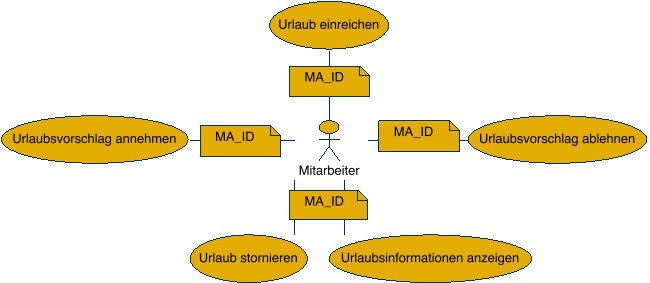
\includegraphics[width=\linewidth]{UML/Export/Urlaub_planen.png}
	\caption{Anwendungsfalldiagramm zur abstrakten Funktion \textit{Urlaub planen - Mitarbeiter}}
	\label{Urlaubplanen}
\end{figure}

\newpage

\section{Detaillierte Beschreibung der essentiellen Funktionalität \textit{Urlaub beantragen}}
Die essentielle Funktion \textit{Urlaub beantragen} geh\"ort zu den kleinsten von anderen unabh\"angigen Anwendungsf\"allen. Beschreiben kann man sie wie folgt: \newline 

Der Mitarbeiter verfasst seinen Urlaubsantrag, basierend auf seinen aktuellen Urlaubsinformationen. Der Antrag enth\"alt die Daten MA-ID, Nachname, Vorname und eine Liste der zu beantragenden Urlaubstage. \newline 

Nach \textsc{Chris Rupp} beschreibt man den Anwendungsfall alternativ unter Zuhilfenahme von Schatzschablonen folgenderma{\ss}en: \newline

\textit{SW-System ``Arbeitszeit erfassen und auswerten`` muss dem Mitarbeiter die Möglichkeit bieten Urlaub einzureichen.} \newline

\newline
Eine weitere Detaillierte Form der Modellierung bietet das Aktivit\"atsdiagramm. Es stellt die einzelnen Aktionen dar, die in einer Funktionalit\"at gekapselt sind. Im Fall der essentiellen Funktionalit\"at \textit{Urlaub beantragen} ist das Aktivit\"atsdiagramm trivial, dargestellt in Abbildung \ref{Aktivitaet}

\vspace{1cm}
\begin{figure}[hbp]
	\centering
	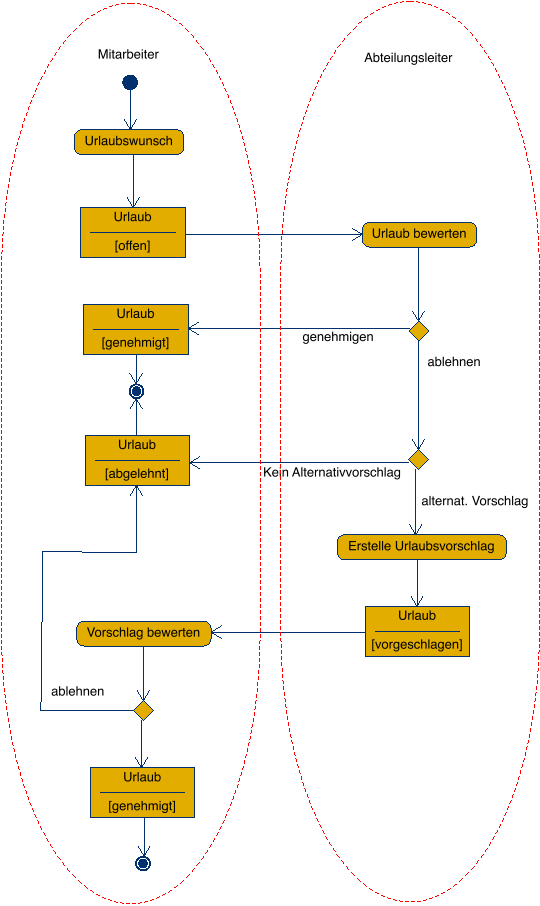
\includegraphics[width=\linewidth]{UML/Export/Urlaub_einreichen.png}
	\caption{Aktivit\"atsdiagramm der essentiellen Funktion \textit{Urlaub beantragen}.}
	\label{Aktivitaet}
\end{figure}

\chapter{Zustandsdiagramm eines Urlaubsantrages}
Der Anwendungsfall \textit{Urlaub planen} eines Mitarbeiters soll nun erneut detaillierter betrachtet werden. Dazu greifen wir das Objekt \textit{Urlaubsantrag} heraus und beschreiben es in einem Zustandsdiagramm genauer. Dieses Diagramm enth\"alt die verschiedenen Zust\"ande einer Betrachtungseinheit und beschreibt gleichzeitig die \"Uberg\"ange zwischen den Zust\"anden.  

\vspace{1cm}
\begin{figure}[hbp]
	\centering
	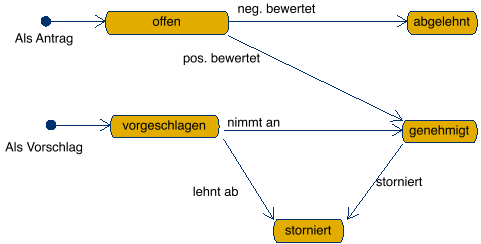
\includegraphics[width=0.9\linewidth]{UML/Export/Urlaubsantrag.png}
	\caption{Zustandsdiagramm des Objekts \textit{Urlaubsantrag}.}
	\label{Uantrag}
\end{figure}

\newpage

\chapter{Entity Relationship Model}
ERM etc. TODO: Leonard

\begin{figure}[hbp]
	\centering
	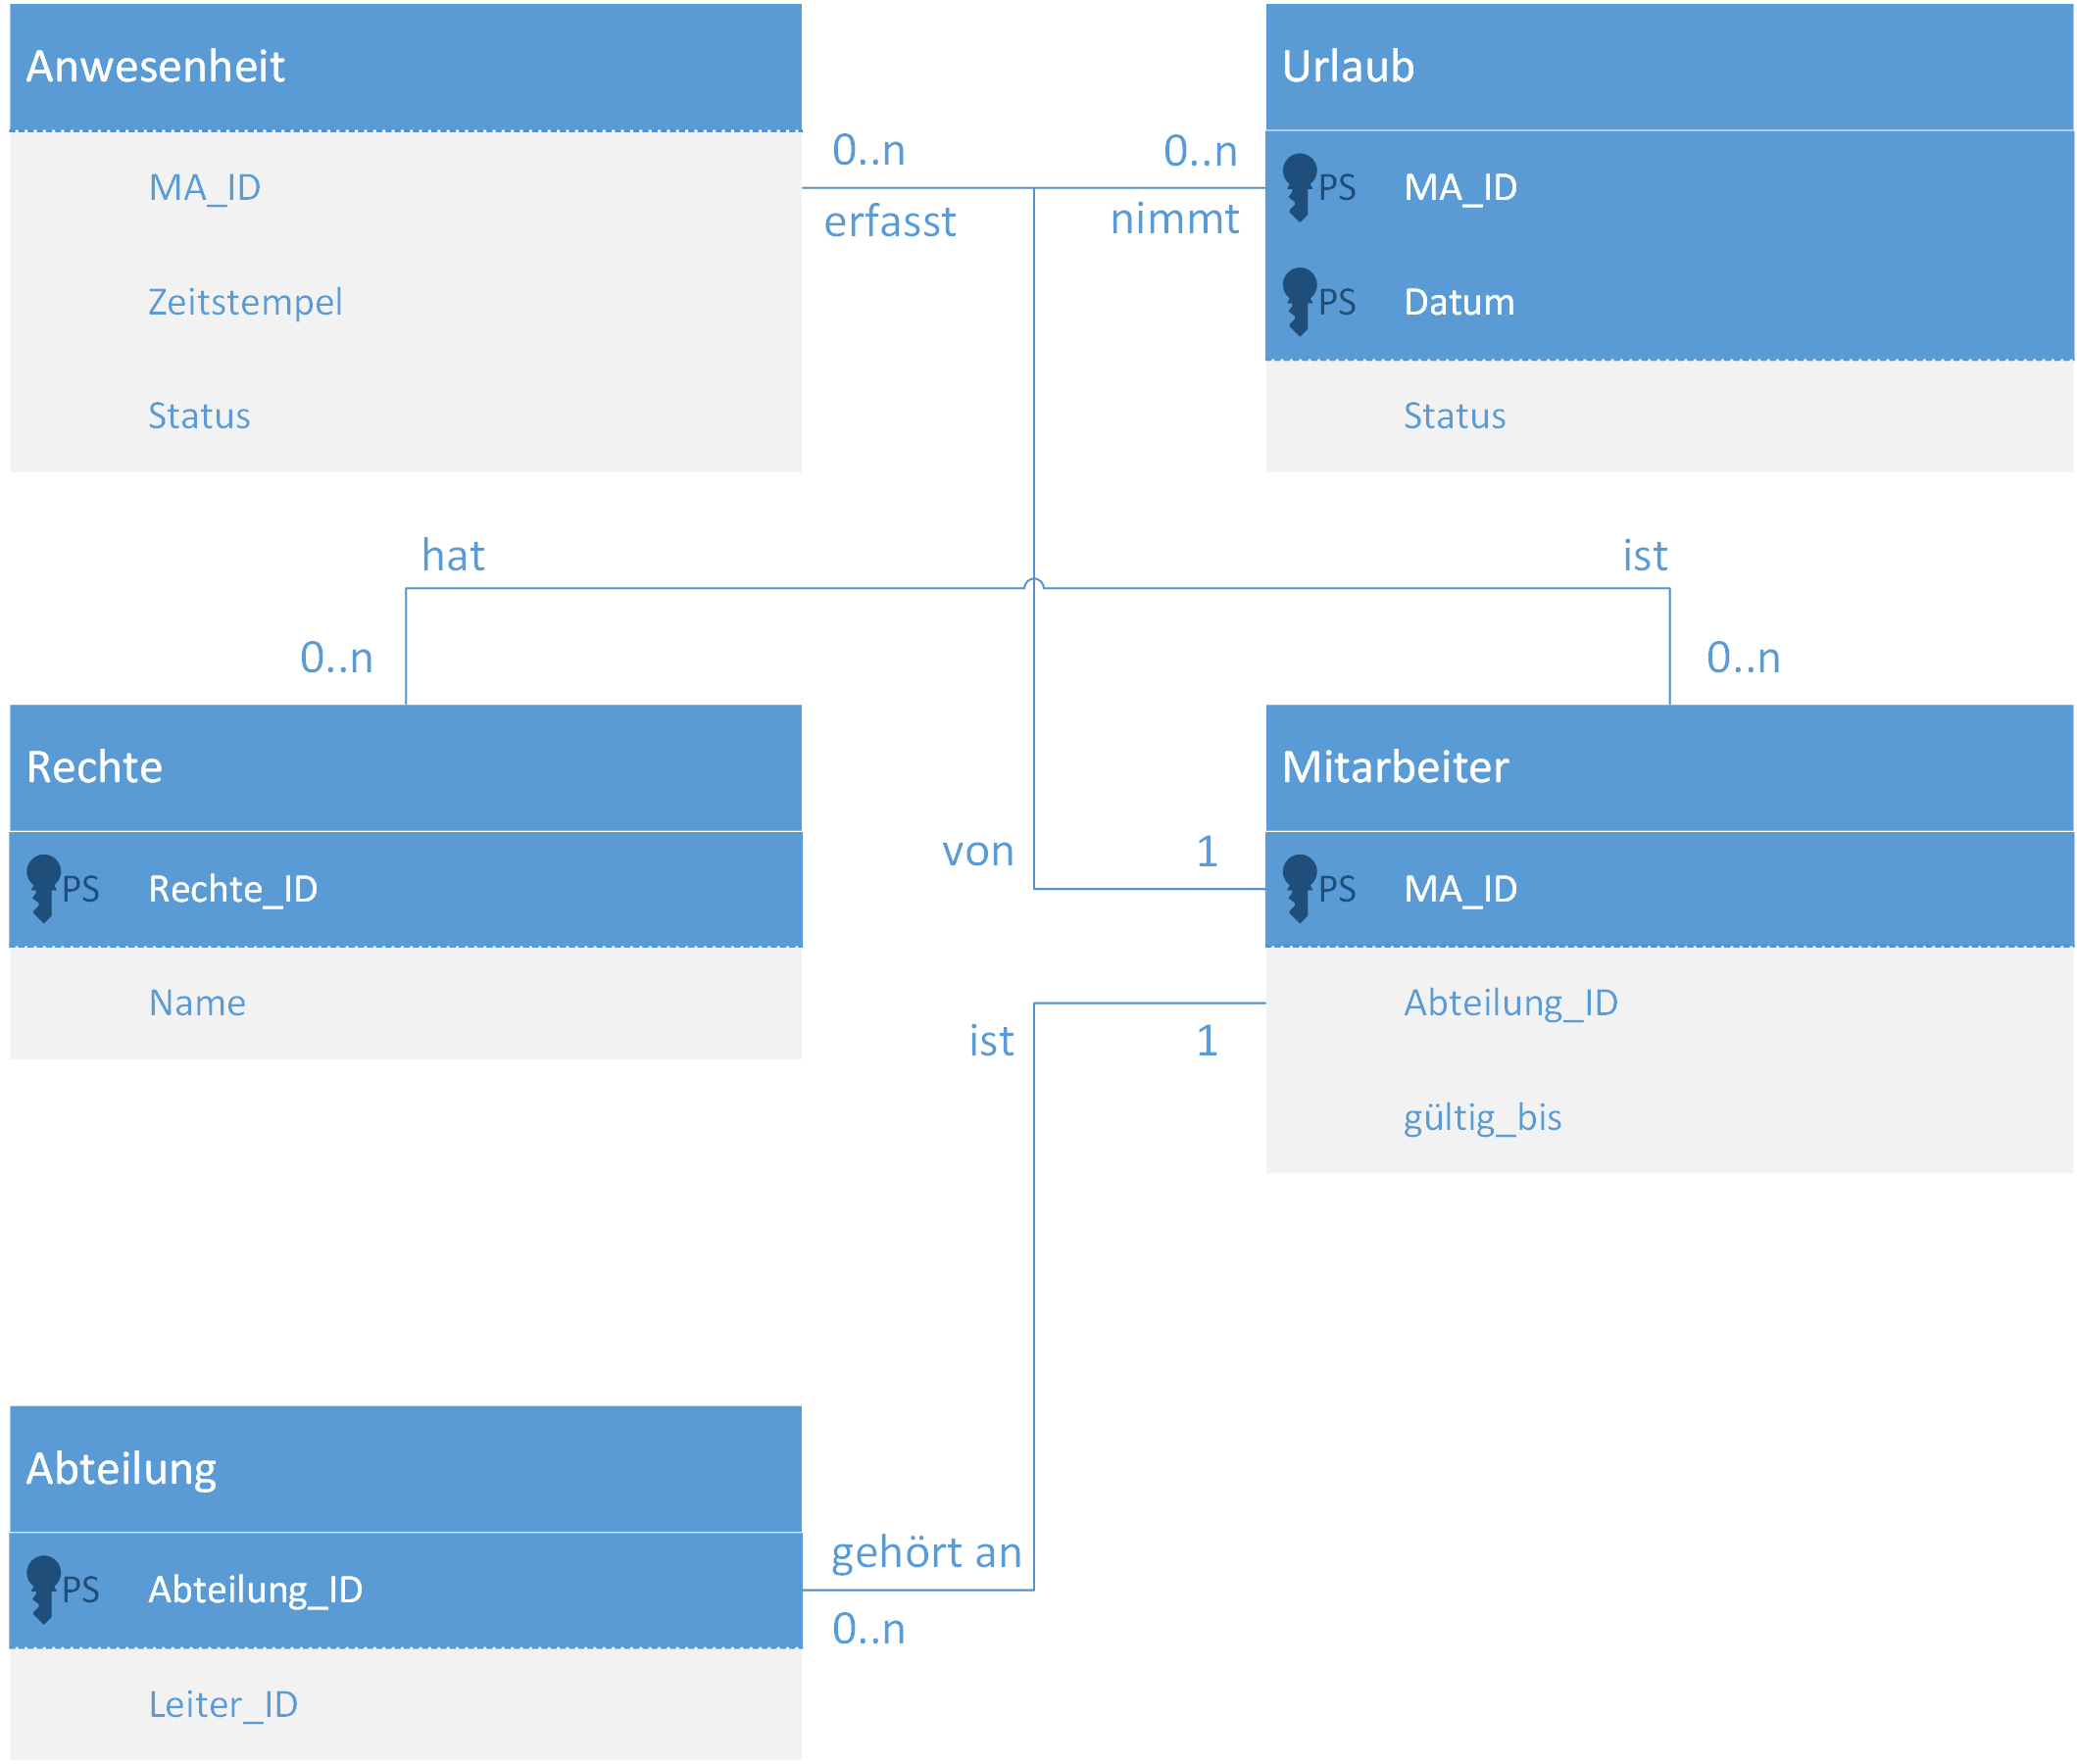
\includegraphics[width=1\linewidth]{UML/Export/erm.png}
	\caption{TEST}
	\label{ERM}
\end{figure}

\chapter{Glossar}
Der abschlie{\ss}ende Glossar soll es Personen aus verschiedenen Fachgebieten m\"oglich machen, die vorliegende Anforderungsanalyse zu verstehen und mit ihr arbeiten zu k\"onnen. Dazu werden wichtige Fachbegriffe aus dem Kontext des Software Engineering und der Anforderungsanalyse beschrieben.

\paragraph{Anwendungsfall}
Eine abstrakte Darstellung einer vom Software-System angebotenen Funktionalit\"at (Aktivit\"at). Er kapselt eine Menge von Aktionen, die sequentiell, bediengungsabh\"angig oder zyklisch abgearbeitet werden. Ein Anwendungsfall wird in Folge von Dateneingaben oder zeitlichen Ereignissen auslegt\"ost und f\"uhrt in der Regel zu einem von au{\ss}en sichtbarem Ergebnis.

\paragraph{Anwendungsfalldiagramm}


\begin{itemize}
	\item 
	\item abstrakte Funktion
	\item essentielle Funktion
	\item Entity Relationship Model
	\item Unified Modeling Language
	\item Mitarbeiter-ID
	\item t.b.c
	\item
	\item 
\end{itemize}


\end{document}
